\documentclass[conference]{IEEEtran}
\usepackage{blindtext, graphicx, caption, subcaption, cite}

\begin{document}
\title{Current Trend in Machine Learning Algorithms and Application on
Health Sensor Data}
\author{\IEEEauthorblockN{Anjana Tiha}
\IEEEauthorblockA{Department of Computer Science\\
University of Memphis, Memphis, TN\\
Email: atiha@memphis.edu}}

\maketitle

\begin{abstract}
This paper is focused with currently trending machine learning algorithms(deep learning, Hierarchical temporal memory) and their application in health sensor data. Also, it captures some of the challenges faced during application of machine learning algorithms and also focuses on some advantages and limitations in applying specific machine learning algorithms in health sensor data. Lastly, it covers focuses on sensor big data and machine learning integration.
\end{abstract}

\begin{IEEEkeywords}
Machine Learning, Trending Machine Learning Algorithms, Deep Learning, Hierarchical Temporal Memory, Distributed Cloud Computing, Spark, Health Sensor Data, Mobile Health.
\end{IEEEkeywords}
\IEEEpeerreviewmaketitle

\section{Introduction}
Machine learning is rapidly growing field of research in computer science. Recently, many new machine learning algorithms are emerging and being applied to diverse fields including interdisciplinary fields. ML is also very popular in mobile health and sports medicine field. Machine learning has been applied on mobile health data for many classification and clustering tasks like activity recognition(like eating, sleeping, walking, running and other sports activities), physiological bio marker detection(stress, smoking detection) and emotion recognition. Among recent machine learning algorithms, Deep Learning is becoming very popular and is assumed to be very powerful and promising. It has been applied in health sensor data with promising result. For example, for activity detection deep learning has worked really well. Hierarchical Temporal Memory(HTM) is also another notable and newly emerging machine learning algorithm which is good at dealing with sequential data. Hierarchical Temporal Memory(HTM) has been used extensively for activity detection on sensor data. In this paper, mainly this two algorithms, their variants and applications have been focused. Other models like random forest and decision tree has long been used for activity classification. Also, Support Vector Machine has been used in many mobile health application like stress detection and smoking prediction.\\
\section{Challanges faced in Health Sensor Data Analysis}
In mobile health and sports health, Machine learning models have been very popular in developing application. But due to specific characteristics of sensor data, application of machine learning models is quite challenging. The process of developing a successful outcome or detection/prediction application is a chain of raw data cleaning, data preprocessing, finding and computing useful features, applying appropriate machine learning models on calculated features and performance analysis with appropriate metrics. Though a big part of sensor data analysis deals with preprocessing raw sensor data to reduce noise, anomaly and identifying proper features, applying most useful machine learning model is also a very important task. Due to task specific challenges, all machine learning algorithms are not suitable for most of all tasks. For example, for activity detection HTM might be more useful, then other algorithms due to sequential nature of activity data. So, exploring and finding out the most useful and appropriate machine learning algorithm for specific task and data is quite important. Also, extracting extract useful features from very large, noise prone dataset is quite challenging. The challenges faced in field of mobile health is also due to added demand for future scalability adaptation and optimization for large dataset. But, adaptation to a population scale data set is very challenging as the huge amount of training data requires outstanding hardware capacity, which is often not feasible and quite impossible. Therefore, scaling the models such that the training can be done on remote machine or distributed on cloud is more proper adaptation. In this paper, big data adaptation for health sensor data would be discussed.
\section{Popular Machine Learning Models}
\subsection{Deep Learning}
Deep Neural Network has been applied in many real word data application and works specially well in presence of large sample size. It has provided good results in terms of prediction and regression though it has reputation for being a black box. Although it gained attention from researchers in recent years, it has been existent before 80’s, but stayed unexplored for decades due to the difficulty of implementation constrains like  hardware limitation and also for popularity of other concurrent ML algorithms like Genetic Algorithm. But with increase of computational capacity and improvement in computing technology, it has has recently gained more attention from researchers.\\
Deep neural network has been inspired by human brain. The model tries to mimic the neuron activity of brain. At neurons the activation occurs  during learning by accumulating previous experience and responses. Similarly, in deep learning sigmoid function are used as activation function at each neurons of deep neural network.\\
\emph{General Architecture:}\\
Deep Neural Network(DNN) is a special type of neural network with numerous hidden layers. Each layer can consist of any number of neurons except output layer which is 1 neuron for classification problems. From the Input Layer (Visible Layer), inputs are passed with a weight to all neurons in the next layer. Then intermediate output for each neuron is computed using input from previous layer, their respective weights and by applying activation function(eg. sigmoid function) at each neuron. When it reaches the output layer, the error is calculated and back propagated to previous layers. Deep Neural Network usually has  numerous hidden layers.
\begin{figure}[h]
\begin{center}
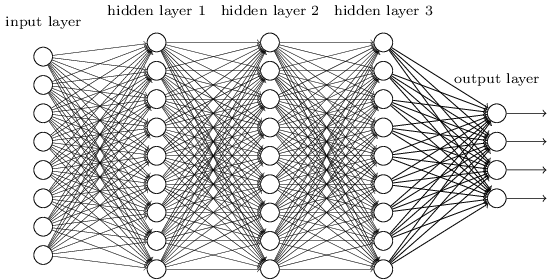
\includegraphics[scale=.4]{DNN}
\end{center}
\caption{Deep Neural Network(DNN)}
\end{figure}\\\\
\emph{Types of Neural Networks:}\\\\
Various deep learning architectures such as like Convolutional Network, Deep Belief network, Recurrent Neural Network are available. Following are some of the popular DNNs.\\
\subsubsection{Convolutional Neural Network}
Convolutional Neural Network is a Multi-layer deep neural network. General deep learning algorithm does not work well for image classification and object detection. Images usually consists of thousands of pixels or even more. For classification or other analysis, each pixel has to be analyzed. For a 200*200-pixel image, at each neuron and for each pixel there will be a large number of weight, so for each layer the computation cost will be very high for even the smallest image size. Convolutional neural network, reduces and optimizes computaional cost for image analysis. Convolutinal Neural Network can also work on audio data or any other data that can be represented as image.\\\\
\emph{Architecture:}\\
Convolutional Neural Network has 4 units: Convolution, Pooling, ReLu, Fully connected layer.\\\\
\emph{Convolutional Layer:} Convolutional Deep Neural network treats image as 4D Data, where along three dimensions, the RGB channel resides and on one dimension weights resides. For full input space, a set of filters with limited receptive field is applied. The filter slides along the height and width of the image. At each pass of each filter, a dot product between the filter and receptive field is calculated and saved in an activation map for their respective filter and receptive field. By combining the activation map for input image space for each filter and stacking them along the depth dimension, output is produced which is input for the next layer.
\begin{figure}[h]
\begin{center}
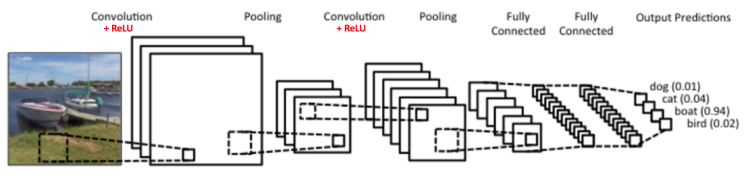
\includegraphics[scale=.7]{CNN}
\end{center}
\caption{Convolutional Neural Network(CNN)}
\end{figure}\\\\
\emph{Pooling layer:} This layer reduces the data size by downsampling. First, it divides the image into equal sized non-overlapping rectangles. Then, pooling function is applied to down sample from each rectangle. The concept is that absolute position is less important than relative position. Many pooling functions are available, but most popular is Max poling which has filter size of 2x2 and from 4 samples 1 highest is chosen, thus reducing the sample size by 75$\%$. Other pooling functions like average is also available but is less effective than max pooling. Usually a pooling layer is sandwiched between few successive convolutional layer. But recently smaller filter size is used instead of using pooling layer.\\\\
\emph{Rectified Linear Unit layer:} Rectified Linear Unit layer (ReLu) is a activation layer. ReLu uses mostly f(x)=max(0,x) fucntion for activation. Other functions like sigmoid and hyperbolic tangent is also applied. But max function is more efficient in terms of computation. This layer try to introduce non linearity.\\\\
\emph{Fully Connected Layer:} Several Convolutional, Pooling Layers can be stacked to develop deep fully connected layer. A Fully connected layer has all the connection to the previous layers and their activation maps. So, they can compute matrix multiplication with bias.\\\\
Lastly, based on the derived output value in the output layer, votes are given for each image for each class. Image with maximum number of votes for candidacy of a class gets classified as the image that class.\\\\
\emph{Application of CNN in health sensor data:}
Convolutional Neural Network is applied in activity detection in Zeng's paper "Convolutional neural networks for human activity recognition using mobile sensors."\cite{Zeng}\\
\subsubsection{Deep Belief Network (DBN)}
Deep Belief Network(DBN) is a graphical model that learns deep hierarchical representation of training data. It is said to be a network where Restricted Boltzmann Machines(RBM) are stacked. It contains sub-networks composed of undirected RBM and directed Bayesian network. Each sub-net is a mixture undirected and directed connections. First layer is trained as an RBM which models raw input as it's visible layer. Using first layer DBN obtains a representation of the input for second layer. Representation can be mean activation or samples, which are the two most common approaches. Now DBN trains the second layer as an RBM, using transformed data (samples or mean activations) as training examples. The above steps can be repeated for the required number of layers. Here, each layer learns all input which is more efficient than shallow network. When trained unsupervised DBN can function as feature generators, in supervised learning, DBN can perform classifications.
\begin{figure}[h]
\begin{subfigure}[b]{0.4\textwidth} 
  \centering
  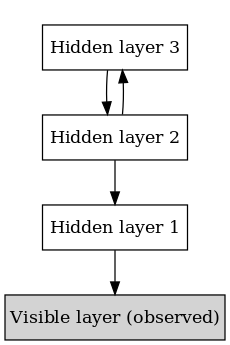
\includegraphics[scale=.4]{DBN2}
  \caption{Deep Beilef Network (DBN)}
  \label{fig:dbn2}
  \end{subfigure}
\end{figure}\\\\
\emph{Application of DBN:}\\
Deep Belief Network has long been applied for human activity recognition. Recently Tamilselvan\cite{Tamilselvan} has used Deep Belief Network for Health Diagnosis Classification. In "Modeling physiological data with deep belief networks" \cite{Wang}, Wang applied DBN to a multimodal dataset with EEG and peripheral physiological signals of 40 subjects for prediction of human affective(emotional) states. In this paper, DBNs was applied to raw physiological data to predict the levels of arousal, valence, and liking, respectively. They have stated that  unsupervised DBNs are capable of learning important features and supervised DBN can obtain good classification performance which is comparable to  Gaussian Naïve Bayes classifiers on hand-crafted features.\\\\
\emph{Popular Market Applications:} Amazon’s Alexa and Apple’s Siri.\\\\
\emph{Advantages and Drawbacks:}\\
The major benefit of Deep Learning technique is, it can be made to work without any domain knowledge from data scientists. With increasing need for application of machine learning in diverse fields, it is becoming increasingly difficult for one to have domain knowledge of so many fields. So, using Deep learning reduces the need and helps making the application of machine learning easier on data scientists. DNN also generates features by itself. So, need for hand crafted feature extraction can be reduced by using DNN. Deep learning is especially helpful in Big Data where data is usually unlabeled and unstructured. It is almost impossible to manually generate features from such huge data and having enough domain knowledge of all data is nearly impossible. Deep learning also reduces need for regularization, since DNN works better than existent popular regularizers like l - 2, l - 1. Deep learning is used to extract and regularize features. Then the extracted regularized features can also be used in training with other machine learning models.\\
The draw backs of the deep neural network are that DNN requires huge amount of data. It is also computationally expensive, for example, model training may take from hours to days or more. So, without using high capacity processing units (like GPUs), it is nearly impossible to implement. Also, finding the right model architecture is very difficult.
\subsection{Herarchical Temporal Memory(HTM)}
Hierarchical temporal memory (HTM) is a machine intelligence which is inspired by neuron activity of  human brain. HTM is a learning algorithms that can store, learn, infer and recall sequential data. It can learn time-based patterns in unlabeled data on a continuous basis. HTM is robust machine learning algorithm which is robust to noise and is capable of learning multiple patterns simultaneously.  Common application includes anomaly detection, classification and ultimately health sensor data applications.
\begin{figure}[h]
\begin{center}
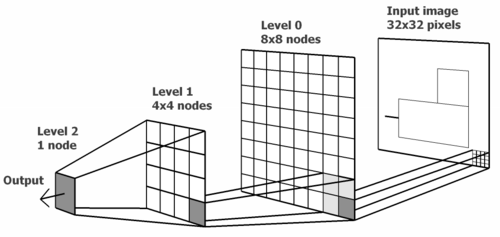
\includegraphics[scale=.4]{HTM}
\end{center}
\caption{Hierarchical Temporal Memory(HTM)}
\end{figure}
HTM network is a tree-shaped hierarchy of levels which are composed of smaller nodes. A single level in the hierarchy is also called a region. The higher in the tree has fewer nodes, has limited power. Often higher level can reuse patterns used in lower levels and by combining them, more complex patterns can be learned.
All nodes in HTM has same functionality. There is usually only one top node. From bottom nodes, the sensor data is feed into HTM. Each higher level node get generalized information from lower level nodes by applying function on input data from output of lower level node. The higher the level is reached the more generalized the information becomes. So, highest level has fewer nodes which is usually one. At each node, the input bits and memorized information from lower level is utilized for arriving at some intermediate conclusion. So, it is well suited for data which is time series/sequential and can be efficient in finding sequential pattern.\\
\emph{Application: }Human activity recognition and other time series data. HMM and HTM has been seen to be very successful detecting activities from sensor data. As the activity detection requires more sequential information and HMM and HTM seems to be a very good fit for sensor data. Also, using deep learning for automated feature calculation has been implemented in many recent papers.
\section{Big Sensor Data and Machine  Model Integration}
Cloud is more appropriate platform for handling big data. It is more suitable for big health sensor data. With development of cloud platform(spark), its very convenient to distribute enormous training tasks to different machines on remote location. But, popular cloud technology like Spark is often not equipped with all modules in their current library to handle all necessary machine learning models. For example, rbf kernel of Support Vector Machine which is very popular, has not yet been integrated in Spark machine learning library "ML-Lib". So, integrating additional machine learning models in the cloud platform(e.g. spark) would be very helpful for research purpose and big data applications. Amount of data is increasing significantly these days. Machine Learning on such big dataset is impossible without distributed architecture. But, integration of new models is also challenging due to structure of cloud. But adaptation could be employed to be more accomodating for new or additional models. For to train a model with Support Vector Machine rbf kernel for a list of hyper parameters, SVM rbf kernel of scikit-learn can be paralleled using custom Grid Search implementation or Random Grid search. I have tried implementing parallel training of SVM for rbf kernel for existent stress detection where almost 200000 parameter combinations can be paralleled using custom Grid  Search and Random Grid Search. There are other efficient solution for many other newer algorithms in Spark also.
\section{Applications}
Deep learning has been used in many diverse datasets. But DNN has specially been successfully used in image classification and speech recognition, semantic and sentiment analysis. It has proven to be more successful than other existent machine learning techniques for certain tasks. In image recognition, it has been documented to outsmart the human. There are different deep learning techniques. Many of them work better on specific fields like, for image and object classification - Convolutional Neural Network works really well. While for activity detection, Deep Belief Network performs well and for natural language processing Recurrent Tensor Network is most popular.
\subsection{Human Activity Detection}
Human activity detection is a popular area of research for sports fitness medicine journals. Using various body sensors like accelerator, gyroscope, magnetometer and different placement of sensors like on wrist, chest, arm, waist or knee, it is possible to recognize human motion and activity. Some of the popular features for activity detection are statistical features like mean, median, percentile, percentile of mean and median, kurtosis, skewness etc. and power spectrum features like power density. Machine learning models that are currently widely used for activity detection are Support Vector Machine, Random Forrest, Decision Tree. But recently Hidden Markov Model(HMM), Hierarchical Temporal Memory(HTM) and last but not least Deep learning is gaining popularity.
\begin{figure}[h]
\begin{center}
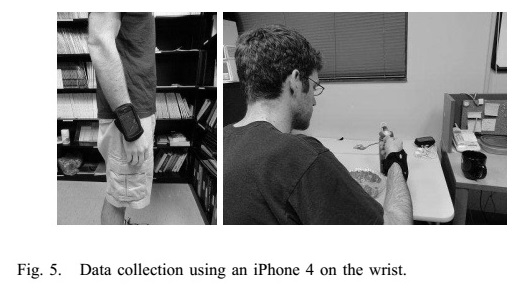
\includegraphics[scale=.6]{ADL}
\end{center}
\caption{Human Activity Recognition(ADL)[Data Collection]}
\end{figure}
\subsection{Eating/Drinking Detection}
Recently, the interest to specific activity like eating and drinking detection has peaked. Eating and drinking detection could help combat obesity and drinking problems in population by identifying and predicting possible drinking activity or eating session. For detection of eating or drinking various combination of sensors has been used similar to activity recognition. But in addition to motion sensors, more audio or utensil sensing has been added in many cases. More accurate and successful works was carried out by using multiple heterogeneous sensors on different body locations. But recent works focuses on detection of eating and drinking using one or the least number of sensors for user convenience which requires more efficient model for learning. Similar to activity detection, eating and drinking detection uses statistical features like mean, median, skewness, kurtosis and percentile, energy, power, percentile of features. Recently, HTM has been used for eating detection.
\subsection{Emotion Recognition}
Various forms of data have been used to recognize emotion. Videos, mobile usage pattern, voice have been able to correctly identify emotion. For emotion cognition from image or videos, Convolutional Neural Network(CNN) is very popular and efficient in human emotion recognition.
\subsection{Stress and Smoking detection}
Stress has been detected with high accuracy from statistical features using Support Vector Machine in paper "cStress: towards a gold standard for continuous stress assessment in the mobile environment" from Hovsepian. Smoking session has also been detected and predicted using SVM. 
\section{Conclusion}
Many novel machine learning algorithms are emerging in the field of machine learning which are capturing attention of researchers. Specially, Deep Neural Network seems to be promising and bringing out interesting advancements in the machine learning field. Though applying machine learning on big data is still a challenge, creative approaches to handle such challenges are emerging. Also, for health data, novel and interesting application of machine learning algorithms seems to be trending in current times. Many newer approaches are introduced to handle current shortcomings and limitations of existing models. 

\begin{thebibliography}{1}
\bibitem{Zeng}
Zeng, Ming, et al. "Convolutional neural networks for human activity recognition using mobile sensors." Mobile Computing, Applications and Services (MobiCASE), 2014 6th International Conference on. IEEE, 2014.
\bibitem{Tamilselvan}
Tamilselvan, Prasanna, and Pingfeng Wang. "Failure diagnosis using deep belief learning based health state classification." Reliability Engineering \& System Safety 115 (2013)$:$124-135.
\bibitem{Wang}
Wang, Dan, and Yi Shang. "Modeling physiological data with deep belief networks." International journal of information and education technology (IJIET) 3.5 (2013)$\:$ 505.
\bibitem{Hovsepian}
Hovsepian, Karen, et al. "cStress: towards a gold standard for continuous stress assessment in the mobile environment." Proceedings of the 2015 ACM international joint conference on pervasive and ubiquitous computing. ACM, 2015. 
\bibitem{Bao}
Bao, Ling, and Stephen S. Intille. "Activity recognition from user-annotated acceleration data." International Conference on Pervasive Computing. Springer Berlin Heidelberg, 2004.
\bibitem{Mannini}
Mannini, Andrea, et al. "Activity recognition using a single accelerometer placed at the wrist or ankle." Medicine and science in sports and exercise 45.11 (2013): 2193.
\bibitem{Zhang}
Zhang, Shaoyan, et al. Physical activity classification using the GENEA wrist-worn accelerometer. Diss. Lippincott Williams and Wilkins, 2012.
\bibitem{Dong}
Dong, Yujie, et al. "Detecting periods of eating during free-living by tracking wrist motion." IEEE journal of biomedical and health informatics 18.4 (2014): 1253-1260.
\end{thebibliography}
\end{document}


